%%%%%%%%%%%%%%%%%%%%%%%%%%%%%%%%%%%%%%%%%%%%%%%%%%%
%% Modèle de rapport pédagogique, doublé d'un tutoriel LaTeX
%% Vincent Labatut 2014-20 <vincent.labatut@univ-avignon.fr>
%%%%%%%%%%%%%%%%%%%%%%%%%%%%%%%%%%%%%%%%%%%%%%%%%%%
%% Classe du document
\documentclass{ceri/sty/rapport}
% \documentclass[handout]{ceri/sty/rapport}
% \documentclass[light]{ceri/sty/rapport}
% \documentclass[full]{ceri/sty/rapport}
% \documentclass[blue]{ceri/sty/rapport}






%%%%%%%%%%%%%%%%%%%%%%%%%%%%%%%%%%%%%%%%%%%%%%%%%%%
%% Informations générales
%%%%%%%%%%%%%%%%%%%%%%%%%%%%%%%%%%%%%%%%%%%%%%%%%%%
%TODO Formation concernée : à compléter.
% Exemples : Licence d'Informatique, Master d'Informatique.
\major{Actuaría}

%TODO Parcours ou spécialité de la formation
% Exemples pour la licence : Systèmes et Réseaux Informatiques, Ingénierie Logicielle.
% Exemples pour le master : Ingénierie du Logiciel pour la Société Numérique, Réseaux Informatiques et Services Mobiles.
\specialization{9no semestre}

%TODO UE concernée par le rapport (à modifier).
% exemple : Projet Algorithmique
\course{Procesos Estocásticos}

%TODO UCE concernée par le rapport (à modifier, optionnel).
\subcourse{FACULTAD DE NEGOCIOS}

%TODO Titre du document, à adapter.
\title{Selección de tema de Proyecto Final}    

%TODO Liste des auteurs
\author{
	Nombre Apellido 
}

%TODO Liste des encadrants, responsables d'UE, etc. (optionnel)
\advisor[Docente]{ % indiquez ici le rôle (par défaut : "Encadrement")
	Jesús E. Batta 
}

%TODO Groupe des auteurs
% Optionnel : seulement si le travail est réalisé en groupe (en l'absence de groupe, ne définissez pas la macro)
% Exemple : Groupe 1, G12, etc.
\group{LAR-963}

% Date de finalisation du rapport. 
% La valeur par défaut, qui est recommandée, est la date du jour.
%\date{\today}

% affiliations des auteurs (pour un rapport de recherche uniquement)
% \affiliations{
%     \textsuperscript{1} Laboratoire Informatique d'Avignon -- LIA EA 4128 \\
%     \textsuperscript{2} Laboratoire Biens, Normes, et Contrats - LBNC EA 3788
% }

% Il est possible de définir un résumé du document (optionnel) avec la commande \resume comme ci-dessous. 
% Si la commande n’apparaît pas, le résumé n'est pas inséré dans le document.
% \summary{Ce document est une introduction à \LaTeX{}. Il s'agit à la fois d'un tutoriel décrivant les principales fonctionnalités de ce système de composition de documents, et d'un modèle servant d'exemple à l'élaboration d'un document. Il utilise le fichier de mise en forme fourni pour l'écriture de rapports dans le cadre des enseignements donnés au CERI, Université d'Avignon.}







%%%%%%%%%%%%%%%%%%%%%%%%%%%%%%%%%%%%%%%%%%%%%%%%%%%
%% Bibliographie
%%%%%%%%%%%%%%%%%%%%%%%%%%%%%%%%%%%%%%%%%%%%%%%%%%%
% Désigne le fichier bibliographique à utiliser
\addbibresource{bibliographie.bib}









%%%%%%%%%%%%%%%%%%%%%%%%%%%%%%%%%%%%%%%%%%%%%%%%%%%
%% Début du document
%%%%%%%%%%%%%%%%%%%%%%%%%%%%%%%%%%%%%%%%%%%%%%%%%%%
\begin{document} 

% Création de la page de titre.
\maketitle

% Justification moins stricte : empêche certains mots de dépasser dans la marge
\sloppy      



%%%%%%%%%%%%%%%%%%%%%%%%%%%%%%%%%%%%%%%%%%%%%%%%%%%
%% INTRODUCCION
%%%%%%%%%%%%%%%%%%%%%%%%%%%%%%%%%%%%%%%%%%%%%%%%%%%
\section{Introducción}
\label{sec:Introduccion}
Este documento es un ejemplo del formato que debe ser empleado en el documento que describirá el tema seleccionado para su proyecto final. En cada una de las secciones se incluye una descripción de las mismas.

\subsection{Contenido de la sección}
La introducción del documento debe permitir que todos los elementos contenidos puedan ser entendidos sin tener un conocimiento experto. Deberán incluirse las referencias correspondientes. Se recomienda que el tema sobre el que desarrollará su proyecto incluya de dos a tres elementos. Es indispensable que al menos uno de estos esté incluido en el temario de la materia de Procesos Estocásticos. Los elementos deberán ser identificados como sub-secciones de la introducción. Al finalizar la sección, se deberá describir de manera rápida cuál será el contenido de cada una de las secciones de su documento. 

\subsection{Especificaciones del documento}
El documento completo debe cumplir con los siguientes requisitos:
\begin{enumerate}
    \item La extensión de todo el documento debe ser menor a las 10 páginas sin considerar la carátula ni la bibliografía. No existe un límite inferior de páginas. 
    \item Las figuras o tablas no pueden presentarse por separado del documento y se deben incluir notas al píe que describan todos los elementos mostrados en la figura o tabla.
    \item Las ecuaciones deben estar numeradas.
    \item El documento tendrá que incluir explícitamente la pregunta de investigación a la que se pretende dar respuesta. Se sugiere que se incluya una sección para este propósito. 
     \item El documento tendrá que incluir explícitamente una sección donde se desarrollen los objetivos, tanto el general como los particulares. El objetivo general debe ser uno solamente. 
    \item El documento tendrá que incluir explícitamente una sección donde se desarrolle la pertinencia de dar respuesta a la pregunta de investigación.
    \item Todas los reglamentos universitarios relativos al plagio son aplicables para este trabajo.
\end{enumerate}

\begin{beware}[Importante]
 Todas observaciones contenidas en este documento deben seguirse para poder obtener los puntos correspondientes de acuerdo a la rúbrica de evaluación del proyecto final.
\end{beware}
 
\subsection{Uso de \LaTeX}
El presente documento es creado a partir de una plantilla en \LaTeX{} \cite{LaTeXProject2010, Wikipedia2011a} distribuida a los miembros del grupo vía Overleaf:
\centerline{\url{https://www.overleaf.com/register}}
\LaTeX{} es un lenguaje para programar el formato de un documento. El código en el que se programa tiene la extensión \texttt{.tex} y el documento que resulta tienen la extensión \texttt{.pdf}. En la última sección de este documento se añade un breve tutorial de las funciones utilizadas. Puede encontrar más información en línea, por ejemplo en WikiBooks \cite{Wikibooks2011}.

%%%%%%%%%%%%%%%%%%%%%%%%%%%%%%%%%%%%%%%%%%%%%%%%%%%%

%%%%%%%%%%%%%%%%%%%%%%%%%%%%%%%%%%%%%%%%%%%%%%%%%%%
%% PREGUNTA DE INVESTIGACIÓN
%%%%%%%%%%%%%%%%%%%%%%%%%%%%%%%%%%%%%%%%%%%%%%%%%%%
\section{Pregunta de investigación}
\label{sec:pregunta}
En esta sección se escribe la pregunta de investigación de su proyecto. En esta sección no es necesario incluir nada más. A continuación se muestra un ejemplo de pregunta de investigación, la cuál debe empezar con \emph{¿Qué?}.

\begin{quote}
    \textbf{¿Qué condiciones son necesarias para que la propiedad de Markov se manifieste en el nivel de aprobación de la cabeza de un gobierno nacional?}
\end{quote}

%%%%%%%%%%%%%%%%%%%%%%%%%%%%%%%%%%%%%%%%%%%%%%%%%%%
%% Objetivos
%%%%%%%%%%%%%%%%%%%%%%%%%%%%%%%%%%%%%%%%%%%%%%%%%%%
\section{Objetivos}
\label{sec:Generalites}
En esta sección se detalla el objetivo general del proyecto, el cuál debe estar relacionado con la pregunta de investigación, y los objetivos particulares, que están relacionados con los pasos que se deben cumplir para concretar el objetivo general. Los objetivos deben estar redactados como oraciones que inicien con un verbo en infinitivo. El objetivo general puede contener uno o dos verbos en infinitivo. Los objetivos particulares deben presentarse de manera secuencial si existe una dependencia entre ellos.
\subsection{Objetivo General}
\begin{quote}
    \textbf{Identificar las características de las series de tiempo de la aprobación del presidente o cabeza de estado que pueden ser representados con modelos de Cadenas de Markov.}
\end{quote}
\subsection{Objetivos Particulares}
\begin{enumerate}
    \item Realizar una categorización de tales series de tiempo por sus características geográficas, políticas, temporales y económicas.
    \item Crear un modelo de cadena de Markov que incluya las características anteriores.
    \item Generar simulaciones del modelo anterior e identificar la discrepancia con los datos reales.
    \item Identificar cual categoría de series de tiempo puede ser representado por una cadena de Markov.
    \item Interpretar el vínculo entre el proceso y el sistema real.
\end{enumerate}
%%%%%%%%%%%%%%%%%%%%%%%%%%%%%%%%%%%%%%%%%%%%%%%%%%%

\section{Pertinencia del tema}

En esta sección se da respuesta a la pregunta ¿Porqué vale la pena responder la pregunta de investigación que estoy planteando? Esta sección estará basada en datos y referencias que evidencien que el tema es relevante y que la pregunta no se ha respondido antes. En la pertinencia del tema debe incluirse información del contexto en el que se plantea la pregunta. 

\section{Herramientas de \LaTeX (Consulte su uso en clase)}
Esta sección no forma parte de los contenidos del documento. Se incluye para mostrar ejemplos de elementos de \LaTeX.

\begin{lstlisting}[language=TeX,numbers=none]

\textbf{Esta instrucción sirve para mostrar código}
\textbf{Por ejemplo, el texto mostrado abajo sirve}
\textbf{para crear la lista de objetivos particulares}
\begin{enumerate}
    \item Realizar una categorización de tales series de tiempo por sus características geográficas, políticas, temporales y económicas.
    \item Crear un modelo de cadena de Markov que incluya las características anteriores.
    \item Generar simulaciones del modelo anterior e identificar la discrepancia con los datos reales.
    \item Identificar cual categoría de series de tiempo puede ser representado por una cadena de Markov.
    \item Interpretar el vínculo entre el proceso y el sistema real.
\end{enumerate}

\end{lstlisting}

\begin{beware}[Importante:]
Puede remarcar la importancia de un párrafo utilizando la opción "beware"
\end{beware}


\paragraph{Color} Puede colorear un texto con el comando \texttt{\textbackslash{}textcolor}:
\textcolor{red}{Ejemplo Rojo} , \colorbox{green}{Ejemplo con fondo verde}.
%%%

\paragraph{Símbolos matemáticos.} Las variables matemáticas deben estar rodeadas por el signo $\$$ cuando se encuentran en una línea. Por ejemplo:  \texttt{\$y = ax + b\$}) genera la expresión $y = ax + b$. En caso de que quiera usar variables matemáticas en un párrafo completo puede escribirlo entre doble signo de pesos ($\$\$ $), entre los símbolos \texttt{\textbackslash{}[ \textbackslash{}]} o usando la instrucción \emph{equation}.


%%%%%%%%%%%%%%%%%%%%%%%%%%%%%%%%%%%%%%%%%%%%%%%%%%%
\paragraph{Estructura}
El texto puede ser estructurado en secciones, sub-secciones, etc. usando instrucciones en \LaTeX. El nivel de jerarquía esta representado en la Tabla~\ref{tab:sections}. 

\begin{table}[htb!]
	\centering
	\rowcolors{1}{fgVeryLightRed}{}
	\begin{tabular}{r l}
		\hline
		\rowcolor{fgLightRed} 
		\textbf{Nivel jerárquico} & \textbf{Comando correspondiente} \\
		\hline
		$1$ & \texttt{\textbackslash{}section} \\
		$2$ & \texttt{\textbackslash{}subsection} \\
		$3$ & \texttt{\textbackslash{}subsubsection} \\
		$4$ & \texttt{\textbackslash{}paragraph} \\
		\hline
	\end{tabular}
	\caption{Commandes utilisées pour définir les titres de sections et sous-sections.}
	\label{tab:sections}
\end{table}

%%%%%%%%%%%%%%%%%%%%%%%%%%%%%%%%%%%%%%%%%%%%%%%%%%%
%% Éléments flottants
%%%%%%%%%%%%%%%%%%%%%%%%%%%%%%%%%%%%%%%%%%%%%%%%%%%

%%%%%%%%%%%%%%%%%%%%%%%%%%%%%%%%%%%%%%%%%%%%%%%%%%%
\subsection{Figuras}
\label{sec:Figuras}

\begin{lstlisting}[language=TeX,numbers=none]
\begin{figure}[htb!]
	\centering
	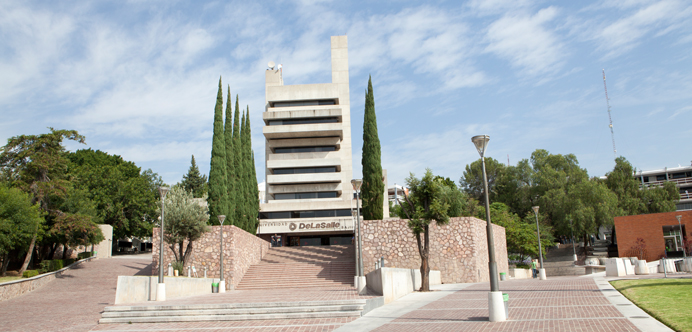
\includegraphics[scale=1]{images/rectoria_ulasalle.jpg}	\caption[Rectoría U LA SALLE]{Fachada de la Rectoría de la Universidad de La Salle Bajío, campus Campestre.}
	\label{fig:uapv}
\end{figure}
\end{lstlisting}
El resultado del código anterior es la Figura~\ref{fig:rectoria}.
\begin{figure}[htb!]
	\centering
	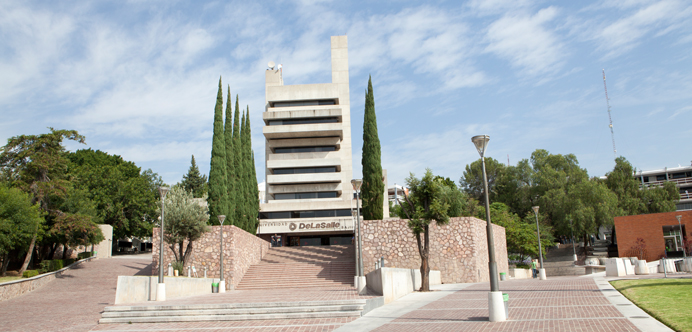
\includegraphics[scale=1]{images/rectoria_ulasalle.jpg}	\caption[Rectoría U LA SALLE]{Fachada de la Rectoría de la Universidad de La Salle Bajío, campus Campestre.}
	\label{fig:rectoria}
\end{figure}

%%%%%%%%%%%%%%%%%%%%%%%%%%%%%%%%%%%%%%%%%%%%%%%%%%%

%%%%%%%%%%%%%%%%%%%%%%%%%%%%%%%%%%%%%%%%%%%%%%%%%%%
\subsection{Ecuaciones}
\label{sec:Equations}

\begin{lstlisting}[language=TeX,numbers=none]
\begin{equation}
	f(s) = h(s) + \max(g_1(s), g_2(s))
	\label{equ:exemple}
\end{equation}
\end{lstlisting}
La ecuación correspondiente es la siguiente:
\begin{equation}
	f(s) = h(s) + \max(g_1(s), g_2(s)).
	\label{equ:exemple}
\end{equation}

Ejemplo de matrices: 
\begin{equation}
	M = 
	\begin{pmatrix}
		a & b & c \\
		d & e & f \\
		g & h & i
	\end{pmatrix}.
	\label{equ:matrice}
\end{equation}

\begin{lstlisting}[language=TeX,numbers=none]
\begin{equation}
	M = 
	\begin{pmatrix}
		a & b & c \\
		d & e & f \\
		g & h & i
	\end{pmatrix}.
	\label{equ:matrice}
\end{equation}
\end{lstlisting}

%%%
\subsection{Como crear bibliografía}  
\LaTeX{} genera la sección de bibliografía con en comando \texttt{\textbackslash{}MyBibliography}. La lista sigue las convenciones configuradas. Las modificaciones se deben realizar en el archivo \texttt{bibliografia.bib}.


%%%%%%%%%%%%%%%%%%%%%%%%%%%%%%%%%%%%%%%%%%%%%%%%%%%
%% Bibliographie
%%%%%%%%%%%%%%%%%%%%%%%%%%%%%%%%%%%%%%%%%%%%%%%%%%%
\MyBibliography


\end{document}
